%!TEX root = ../msc_thesis.tex

\chapter{Variational Inference}
\label{ch:variational_inference}

%%%%%%%%%%%%%%%%%%%%%%%%%%%%%%%%%%%%%%%%%%%%%%%%%%%%%%%%%%%%%%%%%%%%%%%%%%%%%%%%%%%%%%%%%%
%%%%%%%%%%%%%%%%%%%%%%%%%%%%%%%%%%%%%%%%%%%%%%%%%%%%%%%%%%%%%%%%%%%%%%%%%%%%%%%%%%%%%%%%%%
%%% VI
%%%%%%%%%%%%%%%%%%%%%%%%%%%%%%%%%%%%%%%%%%%%%%%%%%%%%%%%%%%%%%%%%%%%%%%%%%%%%%%%%%%%%%%%%%
%%%%%%%%%%%%%%%%%%%%%%%%%%%%%%%%%%%%%%%%%%%%%%%%%%%%%%%%%%%%%%%%%%%%%%%%%%%%%%%%%%%%%%%%%%

% \section{Variational Inference}

As mentioned before, when doing Bayesian inference, it is of interest to compute the posterior distribution $\prob{\theta | y, X}$, which is very often intractable, so one must resort to numerical approximations. In this chapter, we give a brief overview of one possible numerical approximation, called variational inference (VI). The idea of VI is to use optimization to approximate the target distribution $\prob{\theta | y, X}$ with some other approximate distribution $q(\theta)$ that minimizes the Kullback-Leibler (KL) divergence to the real posterior \cite{blei2017variational}. This divergence is defined as
\begin{equation}
  \label{eq:kl_divergence}
  \kl{q}{p} = \mathbb{E}_q \left[ \log \left( \frac{q(\theta)}{\prob{\theta | y, X}} \right) \right] = \int_{-\infty}^{\infty} q(\theta) \left[ \log \left( \frac{q(\theta)}{\prob{\theta | y, X}} \right) \right] d\theta.
\end{equation}

Note that the KL divergence is not symmetrical, i.e., $\kl{q}{p} \neq \kl{p}{q}$, and that is why it is called a divergence and not a distance. The former is called the reverse KL and the latter is called the forward KL, and each one of them prioritizes different aspects of the approximation. 

% The usual goal is to minimize $\kl{q}{p}$ instead of $\kl{p}{q}$ because the latter requires averaging with respect to $\prob{\theta | y, X}$, which is what the modeler is trying to approximate in the first place. Methods to deal with this type of KL divergence exist and are called expectation propagation, but they are not of concern in this work.

Although the main goal of VI methods is tho minimize the KL divergence in \ref{eq:kl_divergence}, in practice what is usually done is to maximize a related quantity called the ELBO (Evidence Lower BOund), defined as
\begin{equation}
  \label{eq:elbo_def}
  \mathcal{L}(q) = \mathbb{E}_q\left[ \log p(y, X, \theta) \right] - \mathbb{E}_q\left[ \log q(\theta) \right].
\end{equation}

The relationship between ELBO and KL divergence is easy to see. Starting from the KL divergence definition, using the logarithm quotient rule, and by the fact that the expected value is a linear operator, then
\begin{equation}
    \kl{q}{p} =
    \mathbb{E}_q \left[ \log \left( \frac{q(\theta)}{\prob{\theta | y, X}} \right) \right] =
    \mathbb{E}_q \left[ \log  q(\theta) \right] - \mathbb{E}_q \left[ \log {\prob{\theta | y, X}}  \right].
\end{equation}

Then, using the definition of conditional probability,
\begin{equation}
    %\mathbb{E}_q \left[ \log  q(\theta) \right] - \mathbb{E}_q \left[ \log p(\theta | y, X)  \right] =
    \kl{q}{p} =
    \mathbb{E}_q \left[ \log  q(\theta) \right] - \mathbb{E}_q \left[ \log \frac{p(\theta, y, X)}{p(y | X) p(X)}  \right].
\end{equation}

Using the logarithm quotient rule one more time,
\begin{equation}
  % \mathbb{E}_q \left[ \log  q(\theta) \right] - \mathbb{E}_q \left[ \log \frac{p(\theta, y, X)}{p(y | X) p(X)}  \right] =
  \kl{q}{p} =
  \mathbb{E}_q \left[ \log  q(\theta) \right] - \mathbb{E}_q \left[ \log p(\theta, y, X) - \log p(y | X) - \log p(X)  \right].
\end{equation}

But since $p(X)$ does not depend on $q$, the expected value of $p(X)$ is a constant, hence
\begin{equation}
 %\mathbb{E}_q \left[ \log  q(\theta) \right] - \mathbb{E}_q \left[ \log p(\theta, X) - \log p(X)  \right] =
 \kl{q}{p} =
 \mathbb{E}_q \left[ \log  q(\theta) \right] - \mathbb{E}_q \left[ \log p(\theta, y, X) \right] + \log p(y | X) + \log p(X).
\end{equation}

Since the goal is to find the optimal $q$, then $\log p(X)$ is just a constant in the optimization process, and can be ignored to just minimize the equation
\begin{equation}
  \mathbb{E}_q \left[ \log  q(\theta) \right] - \mathbb{E}_q \left[ \log p(\theta, y, X) \right]
\end{equation}
which is the negative of the ELBO. Hence, minimizing the KL divergence is equivalent to maximizing the ELBO.

Let $\lambda$ be the parameters of the variational distribution $q(\theta)$. The objective is to approximate $p(\theta | y, X)$ by finding the values of the $\lambda$ vector that maximize equation \ref{eq:elbo_def}, which could be done in several ways, for example, coordinate ascent, or gradient ascent. In order to perform gradient ascent, is it necessary to compute the gradient of the objective function with respect to the parameters, that is, $\nabla_{\lambda} \mathcal{L}(q, \lambda)$. It is not very hard to prove that
\begin{equation}
  \label{eq:ELBO_gradient}
  \nabla_{\lambda} \mathcal{L}(q, \lambda) =
  \mathbb{E}_q \left[ \left( \nabla_{\lambda} \log q(\theta | \lambda) \right) \left( \log p(y, X, \theta) - \log q(\theta | \lambda) \right) \right].
\end{equation}

There are situations in which this gradient can be computed analytically, but for many other models, this cannot be done because it may not be possible to analytically take the expectation, hence some approximation must be made. A good approach is to approximate the expected value with Monte Carlo simulation. Let $\left\{ z_1, ..., z_S \right\}$ be samples taken from $q(\theta | \lambda)$, then one can approximate the expected value with an arithmetic mean as such,
``````````\begin{equation}
  \begin{split}
  \nabla_{\lambda} \mathcal{L}(q, \lambda) &=
  \mathbb{E}_q \left[ \left( \nabla_{\lambda} \log q(\theta | \lambda) \right) \left( \log p(y, X, \theta) - \log q(\theta | \lambda) \right) \right] \\
  & \approx \frac{1}{S} \sum_{k = 1}^S \left( \nabla_{\lambda} \log q(z_k | \lambda) \right) \left( \log p(y, X, z_k) - \log q(z_k | \lambda) \right).
  \end{split}
\end{equation}

This approach gives noisy but unbiased estimates of the expected value. A Monte Carlo approach can also be taken to compute the value of the ELBO. For more details about this see \cite{kucukelbir2017automatic} and \cite{ranganath2014black}.

A family that is often used to approximate $p$ is the \textbf{mean-field variational family}, where each parameter is independent of the rest, such that
\begin{equation}
  q(\theta) = \prod_{i = 1}^p q(\theta_i | \lambda_i).
\end{equation}

To illustrate this, let's study a simple example in which the goal will be to try to approximate the posterior distribution of a two-class logistic regression. Assume a data matrix $X \in \mathbb{R}^{n \times p}$ and a response vector $y$ with values 1 or 0. Each observation $y_i$ is modeled with a Bernoulli distribution such that
\begin{equation}
  y_i | x_i, \theta \sim \mathrm{Bern}(\sigma(\theta^T x_i))
\end{equation}
where $\sigma(\cdot)$ is the logistic sigmoid function. The prior distribution for $\theta$ is a Gaussian $\theta \sim \normaldist{0}{\sigma_0^2 \mathbb{I}_p}$ where $\mathbb{I}_p$ is the $p \times p$ identity matrix and $\sigma_0^2 \in \mathbb{R}^+$.

In this case, the mean-field variational distribution is
\begin{equation}
  \label{eq:mean_field_normal_prior}
  q(\theta | \lambda) = \prod_{j = 1}^p \normalfunc{\theta_j}{\mu_j}{\sigma_j^2}
 \end{equation}
with $\lambda = \left[ \mu_1, \hdots, \mu_p, \sigma_1^2, \hdots, \sigma_p^2 \right]^T$ and where $\normalfunc{\theta_j}{\mu_j}{\sigma_j^2}$ denotes the value of a normal density function at $\theta_j$ with mean $\mu_j$ and variance $\sigma_j^2$.

According to equation \ref{eq:ELBO_gradient}, to compute the gradient of the ELBO, we need to be able to compute $\nabla_{\lambda} \log q(\theta | \lambda)$, so we need that partial derivative of $\log q(\theta | \lambda)$ with respect to each $\mu_j$ and $\sigma_j^2$, $j \in \left\{ 1, \hdots, p \right\}$. Let's start with $\mu_j$.
\begin{equation}
  \begin{split}
      \nabla_{\mu_j} \log q(\theta | \lambda) & =
      \nabla_{\mu_j} \log \left( \prod_{ k = 1}^p \normalfunc{\theta_k}{\mu_k}{\sigma_k^2} \right) \\
      &= \nabla_{\mu_j} \sum_{ k = 1}^p \log \left( \normalfunc{\theta_k}{\mu_k}{\sigma_k^2} \right) \\
      &= \nabla_{\mu_j} \log \left( \normalfunc{\theta_j}{\mu_j}{\sigma_j^2} \right) \\
      &= \nabla_{\mu_j} \log \left( \frac{1}{\sqrt{2 \pi \sigma_j^2}} \exp \left( -\frac{(\theta_j - \mu_j)^2}{2 \sigma_j^2} \right) \right) \\
      &= \frac{\theta_j - \mu_j}{\sigma_j^2}.
  \end{split}
\end{equation}

Now for $\sigma_j^2$. It is easier to work with the logarithm, so let $\alpha_j = \log \sigma_j^2$, and instead of computing $\nabla_{\sigma_j^2}$, $\nabla_{\alpha_j}$ will be computed.

\begin{equation}
  \begin{split}
      \nabla_{\alpha_j} \log q(\theta | \lambda) & =
      \nabla_{\alpha_j} \log \left( \prod_{ k = 1}^p \normalfunc{\theta_k}{\mu_k}{\sigma_k^2} \right) \\
      &= \nabla_{\alpha_j} \sum_{ k = 1}^p \log \left( \normalfunc{\theta_k}{\mu_k}{\sigma_k^2} \right) \\
      &= \nabla_{\alpha_j} \log \left( \normalfunc{\theta_j}{\mu_j}{\sigma_j^2} \right) \\
      &= \nabla_{\alpha_j} \log \left( \frac{1}{\sqrt{2 \pi \sigma_j^2}} \exp \left( -\frac{(\theta_j - \mu_j)^2}{2 \sigma_j^2} \right) \right) \\
      &= \nabla_{\alpha_j} \log \left( \frac{1}{\sqrt{2 \pi \mathrm{e}^{\alpha_j}}} \exp \left( -\frac{(\theta_j - \mu_j)^2}{2 \mathrm{e}^{\alpha_j}} \right) \right) \\
      &= - \nabla_{\alpha_j} \log \left( \sqrt{2 \pi \mathrm{e}^{\alpha_j}} \right) - \frac{(\theta_j - \mu_j)^2}{2} \nabla_{\alpha_j} \mathrm{e}^{-\alpha_j}\\
      &= - \frac{1}{2} + \frac{(\theta_j - \mu_j)^2}{2} \mathrm{e}^{-\alpha_j} \\
      &= - \frac{1}{2} + \frac{(\theta_j - \mu_j)^2}{2 \sigma_j^2}.
  \end{split}
\end{equation}

To compute the gradient in equation \ref{eq:ELBO_gradient}, it is necessary to also compute the log-likelihood of the data $p(y, X, \theta)$. Using the chain rule of probability, this can be written as $\log p(y | X, \theta) + \log p(X | \theta) + \log p(\theta)$. Note that in order to compute the gradient, $\log p(X | \theta)$ is not needed, because of the following
\begin{equation*}
  \begin{split}
      \nabla_{\lambda} \mathcal{L} &=
      \mathbb{E}_q \left[ \left( \nabla_{\lambda} q(\theta | \lambda) \right) \left( \log p(y, X, \theta) - \log q(\theta | \lambda) \right) \right] \\
      &= \mathbb{E}_q \left[ \left( \nabla_{\lambda} q(\theta | \lambda) \right) \left( \log p(y | X, \theta) + \log p(X | \theta) + \log p(\theta) - \log q(\theta | \lambda) \right) \right] \\
      &= \mathbb{E}_q \left[ \left( \nabla_{\lambda} q(\theta | \lambda) \right) \left( \log p(y | X, \theta) + \log p(\theta) - \log q(\theta | \lambda) \right) \right] +  \log p(X | \theta) \mathbb{E}_q \left[ \nabla_{\lambda} q(\theta | \lambda) \right] \\
      &= \mathbb{E}_q \left[ \left( \nabla_{\lambda} q(\theta | \lambda) \right) \left( \log p(y | X, \theta) + \log p(\theta) - \log q(\theta | \lambda) \right) \right] +  c \mathbb{E}_q \left[ \nabla_{\lambda} q(\theta | \lambda) \right].
  \end{split}
\end{equation*}

In the last line, $\log p(X | \theta)$ has been reduced to just a constant $c$. It can be seen that $\mathbb{E}_q \left[ \nabla_{\lambda} q(\theta | \lambda) \right] = 0$ by using the dominated convergence theorem like it was done in \cite{ranganath2014black}.

\begin{equation}
  \begin{split}
      \mathbb{E}_q \left[ \nabla_{\lambda} q(\theta | \lambda) \right] &=
      \int \nabla_{\lambda} q(\theta | \lambda) d\theta \\
      &= \nabla_{\lambda} \int q(\theta | \lambda) d\theta \\
      &= \nabla_{\lambda} 1 d\theta \\
      &= 0.
  \end{split}
\end{equation}

So, the derivative of the ELBO can be written as
\begin{equation}
  \nabla_{\lambda} \mathcal{L} = \mathbb{E}_q \left[ \left( \nabla_{\lambda} q(\theta | \lambda) \right) \left( \log p(y | X, \theta) + \log p(\theta) - \log q(\theta | \lambda) \right) \right].
\end{equation}

Since $y$ is a Bernoulli random vector, then
\begin{equation}
  \begin{split}
      \log p(y | X, \theta) &=
      \log \left( \prod_{i = 1}^n \sigma(\theta^T x_i)^{y_i} (1 - \sigma(\theta^T x_i))^{1-y_i} \right) \\
      &= \sum_{i = 1}^n \left[ y_i \log \left( \sigma(\theta^T x_i \right) + (1 - y_i) (1 - \sigma(\theta^T x_i)) \right].
  \end{split}
\end{equation}

And since $\theta$ was assumed to have Gaussian prior, then
\begin{equation}
  \log p(\theta) = \log \prod_{j = 1}^p \phi(\theta_j) = \sum_{j = 1}^p \log \phi(\theta_j) = \frac{1}{\sqrt{2 \pi}} e^{\left( -\frac{\theta_j^2}{2} \right)}.
\end{equation}

With these derivations, a gradient ascent approach can be taken in order to optimize the ELBO. This is the same as gradient descent presented in chapter \ref{ch:machine_learning}, except that instead of taking the negative of the gradient to move in the direction of maximum descent, the gradient is taken as it is so that the algorithm moves in the direction of maximum ascent. As in gradient descent, the modeler starts with a random $\lambda$ vector, but in this case where the gradient must be approximated with Monte Carlo simulation, in each step $t$ the algorithm takes $S$ samples $z_k$, with $z_k \sim q(\theta | \lambda)$ for $k \in \left\{1, \cdots, S \right\}$. This way the approximate gradient is computed as
\begin{equation}
  \nabla_{\lambda} \mathcal{L} \approx \Delta_{\lambda} \mathcal{L} = \frac{1}{S} \sum_{k = 1}^S \left( \nabla_{\lambda} \log q(z_k | \lambda) \right) \left( \log p(y, X, z_k) - \log q(z_k | \lambda) \right),
\end{equation}
and then the $\lambda$ parameter is updated as $\lambda_{t+1} = \lambda_{t} + \eta_t  \Delta_{\lambda_t} \mathcal{L}$, with each $\eta_t$ chosen accordingly, until a certain stopping criteria is met.

An implementation of this algorithm was made in R with a simulated data set of $n = 500$ data points and $p = 1$ covariate. The response vector was created with the logistic sigmoid function as $y_i = \sigma(\theta_0 + \theta_1 x_i)$, with $\theta_0 = -5$ and $\theta_1 = 5$. The initial value for $\lambda = \left[ \mu_1, \mu_2, \alpha_1, \alpha_2 ]^T \right]$ is zero, for each iteration $S = 50$ Monte Carlo samples are taken to compute the approximate gradient, and the step size $\eta_t$ is chosen using the AdaGrad method in which
$\eta_t = \left( \mathrm{diag}(G_t) \right)^{\frac{1}{2}}$, where $\mathrm{diag}(G_t)$ refers to the diagonal of the matrix $G_t = \left( \Delta_{\lambda_t} \right) \left( \Delta_{\lambda_t} \right)^T$ \cite{duchi2011adaptive}. The stopping criterion is that
% $\frac{\norm{\mu_{t+1} - \mu_{t}}}{\norm{\mu_t}} < 0.00003$,
$\norm{\mu_{t+1} - \mu_{t}} < 0.005$,
with $\mu_t$ being the vector containing the values of $\mu_1$ and $\mu_2$ in the $t$-th iteration of the algorithm.

Figure \ref{fig:BBVI_plots} shows the results of the implementation, and a comparison of the values estimated by the \texttt{glm} package in R is also shown. The top-left image shows the value of the objective function, i.e., the ELBO, in each iteration, slowly increasing and with a wiggly line because of the noise of the estimations. The top-right image shows the real values of $\theta$ (-5 and 5) with gray dashed lines, the values of $\theta$ estimated by the \texttt{glm} package with colored dotted lines, and the approximated values of the variational distribution $q(\theta | \lambda)$. The bottom-left image shows the values of $\mu_1$ and $\mu_2$ in each iteration, with horizontal colored dotted lines showing the estimated values by the \texttt{glm}package; it can be seen how they slowly approach their real values. The bottom-right image shows the values of $\mu_1$ and $\mu_2$ in each iteration in the plane, where the noise of the gradient estimation is seen in the wiggliness of the line; the red dot shows once again the value estimated by the \texttt{glm} package. In general the results are pretty good for such a simple algorithm. There are ways to have better and less noisy estimates, but they are beyond the scope of this work. For more details about better approximations of the gradient, see \cite{kucukelbir2017automatic} and \cite{ranganath2014black}.

\begin{figure}[H]
    \centering
    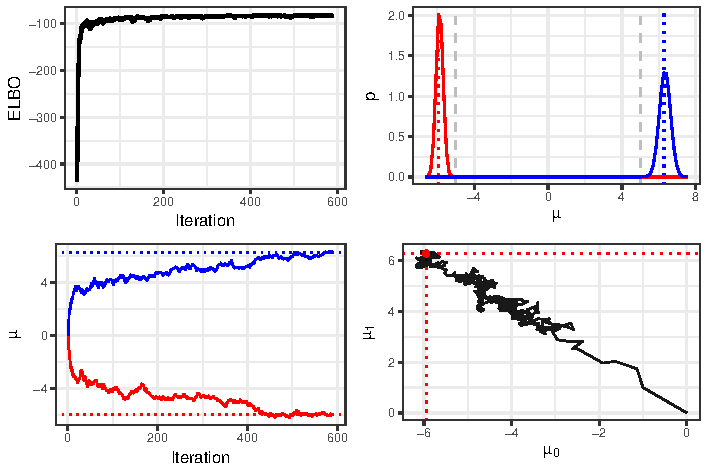
\includegraphics[width=\textwidth]{BBVI_plots.pdf}
    \caption{Example of mean-field variational inference for Bayesian logistic regression.}
    \label{fig:BBVI_plots}
\end{figure}

The posterior predictive distribution of $y^*$ for a new vector of covariates $x^*$ can be approximated using the variational approximation. In particular, the modeler could take $T$ samples from the variational posterior distribution as such, for $j \in \left\{ 1, \ldots, T \right\}$:
\begin{enumerate}
  \item Sample a vector $\theta_j \sim q(\theta | \lambda)$
  \item Use that value to sample $y_j^* \sim p(y^* | \theta_j, x^*)$
\end{enumerate}

Then $\left\{ y_j^* \right\}_{j = 1}^T$ is a set of $T$ independent samples from the posterior predictive distribution $\prob{y^* | y, X, x^*}$.
